\section{Kombinatorik}

\subsection{Produkt}\script{6}
Mit der \textit{Für-jedes-gibt-es-Regel} können $k$ Positionen unabhängig voneinander markiert werden, wobei -n- verschiedene Markierungen zur Verfügung stehen.
\[
P_N = n^k
\]

\subsection{Permutation}\script{7}
Auf wieviele Arten kann man $n$ Objekte anordnen?

\[
P_n = n! = n \cdot P_{n-1}
\]

\subsection{Kombination}\script{8}
Auf wieviele Arten kann man $k$ Objekte aus $n$ auswählen? \textit{Ziehen ohne Zurücklegen}

\begin{align*}
	C_k^n = \frac{n!}{k!(n-k)!} &= \overbrace{\begin{pmatrix}	n \\ k \end{pmatrix}}^\text{Binomialkoeffizieten} \\ \\
	&=  \begin{pmatrix}	n - 1 \\ k -1\end{pmatrix} +  \begin{pmatrix}	n -1\\ k \end{pmatrix} \\
	&= \frac{n}{k} \cdot  \begin{pmatrix}	n - 1 \\ k -1\end{pmatrix}
\end{align*}


\subsection{Erzeugende Funktionen}\script{12}
Idee ist, durch eine Potenzreihe kominatorische Probleme mit algebraischen Manipulationen zu lösen.\\
\textbf{Beispiel:}\\
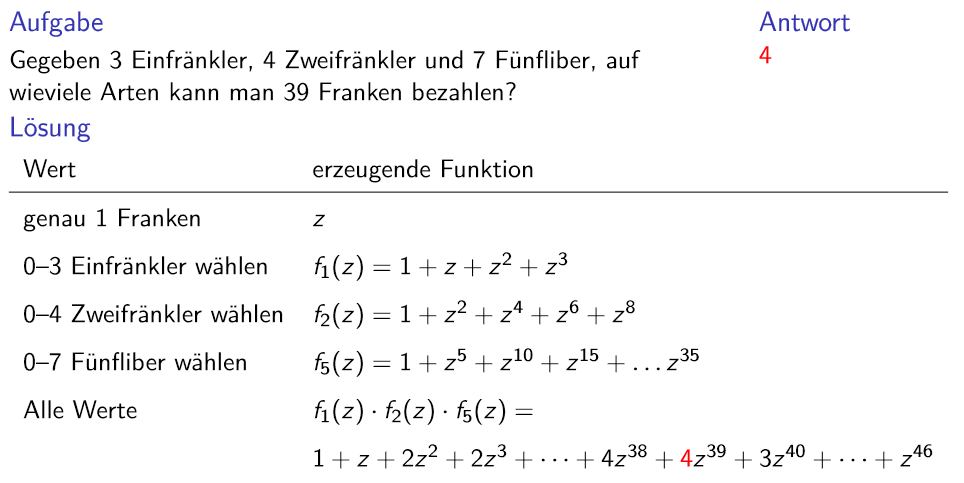
\includegraphics[width=\columnwidth]{Images/erzeugendeFunktion}


\subsection{Ereignisse}
\begin{center}
	\includegraphics[width=0.7\columnwidth]{Images/zählregeln}
\end{center}

\begin{table}[H]
	\centering
	\begin{tabular}{l|l}
		Alle Versuchsausgänge & $\Omega$ \\
		A und B treten ein & $A \cap B$ \\
		A oder B treten ein & $A \cup B$ \\
		nicht A & $\overline{A} = \Omega \backslash A$ \\
		unmögliches Ereignis & $\emptyset$ \\
		A hat B zurfolge & $A \subset B$ \\
	\end{tabular}
\end{table}
\noindent\textbf{Beispiel:} Unfaire Münze $A_k$ erster Kopf im k-ten Wurf mit Anzahl würfeln bis Kopf kommt. Da gewürfelt wird, bis Kopf kommt, ist die Summe aller Wahrscheinlichkeiten $\sum\limits_{k}P(A_k) = 1$.
\[P(A_k) =\underbrace{ p^{k-1}}_{k-1\text{ Würfe ohne Kopf}}\cdot \underbrace{(1-p)}_{\text{k-ter Wurf}}\]


\textbf{Axiome}:\script{34}\\
\begin{align*}
	P(\emptyset) &= 0 \\
	P(\overline{A}) &= P(\Omega \backslash A) = 1 - P(A) \\
	P(A \backslash B) &= P(A) - P(A \cap B) \\
	P(A \cup B) &= P(A)  + P(B) - P(A \cap B) \\
	P(\overline{A} | \overline{B}) &= 1-P(A|\overline{B}) \\
	P(\overline{A} | B) &= 1-P(A|B) \\
\end{align*}

\subsection{Bedingte Wahrscheinlichkeit}\script{39}
Die bedingte Wahrscheinlichkeit eines Ereignisses A unter der Bedingung B. \textit{B ist die neue Gesammtmenge, in welcher A vorkommen kann}:
\[
P(A|B) = \frac{P(A \cap B)}{P(B)} \xRightarrow[\text{S.v. Bayes}]{} P(A|B) = P(B|A)\cdot\frac{P(A)}{P(B)}
\]

\noindent\textbf{Beispiel:} Die Wahrscheinlichkeit, dass ein Raucher (R) Lungenkrebs (L) einwickelt ist $15\%$, Bei Nichtraucher $1\% \rightarrow P(L|R) = 0.15$ und $P(L|\overline{R}) = 0.01$. Wie viel Lungenkrebskrange sind auch Raucher ist unbekannt $P(R|L) = ?$.

\begin{center}
	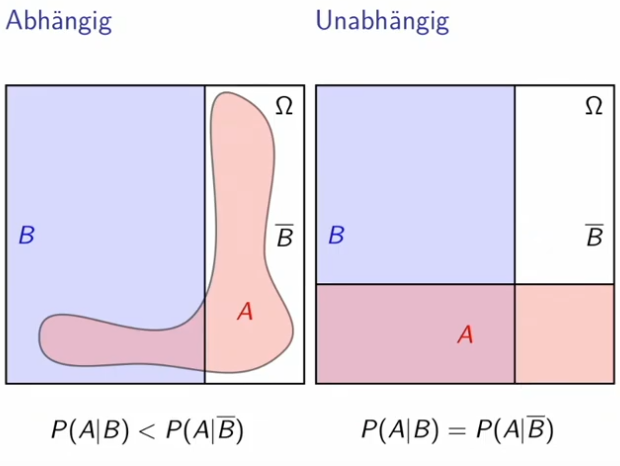
\includegraphics[width=0.5\columnwidth]{Images/bedingte_wahr.}
\end{center}

\noindent Wenn A und B unabhängig sind gilt:
\[ P(A \cap B) = P(A) \cdot P(B)\]


\subsection{Totale Wahrscheinlichkeit}
\[
P(A) = \sum_{n=0}^{m}P(A|B_n)\cdot P(B_n)
\]

\begin{align*}
	P(A) &=P(A|B)P(B) + P(T|\overline{B})P(\overline{B}) \\
	&= P(A|B)P(B) + (1 - P(\overline{A}|\overline{B}))P(\overline{B})
\end{align*}


\subsection{Erwartungswert}\script{60}
Der Erwartungswert $\mu$ einer Zufallsvariable beschreibt die Zahl, die die diese im Mittel annimmt.
\[
\mu = \overline{X} = E(X)= \sum\limits_{i=0}^{n}x_i\cdot \underbrace{P(X=x_i)}_\text{Wr.keit} = \int_{-\infty}^{\infty}x\cdot \underbrace{\varphi(x)}_{\text{Wr.dichte}}dx
\]

\textbf{Rechenregeln} mit Zufallsvariablen $X, Y$:
\begin{itemize}[nosep]
	\item $E(X + Y) = E(X) + E(Y)$
	\item $E(\lambda X) = \lambda E(X)$ 
	\item $E(X\cdot Y) = E(X) \cdot E(Y) \qquad$  (Nur falls Unabhängig)
\end{itemize}

\subsection{Varianz}\script{66}
Die Varianz $\var(X)$ beschreibt die mittlere quadratische Abweichung vom Erwartungswert. Damit lässt sich die Standardabweichung $\sigma$ berechnen.
\begin{align*}
	\var(X) &= E(X^2) - E(X)^2 \\
	&=\sum\limits_{i=0}^{n}(k_i - E(X))^2 \cdot \underbrace{P(X=x_i)}_\text{Wr.keit} \\
	\sigma &= \sqrt{\var(X)}	
\end{align*}

\noindent\textbf{Beispiel} Faire Münze:\\
$P(X = \overbrace{0}^{k_1}) = \frac{1}{2}$, Kopf: $P(X = \overbrace{1}^{k_2}) = \frac{1}{2}$ und der Erwartungswert $E(X)$: 
\begin{align*}
	E(X) &= 0\cdot \frac{1}{2} + 1\cdot\frac{1}{2} = \frac{1}{2} \\
	E(X^2) &= 0^2\cdot \frac{1}{2} + 1^2\cdot\frac{1}{2} = \frac{1}{2}
\end{align*}

\noindent Die Varianz kann auf zwei Arten berechnet werden:\\
\textit{Option1:} $\var(X) = (0 - \frac{1}{2})^2 \cdot \frac{1}{2} + (1 - \frac{1}{2})^2 \cdot 1 \xrightarrow{} \frac{1}{4}$\\
\textit{Option2:} $\var(X) = E(X^2) - E(X)^2 = \frac{1}{2} - \frac{1}{4} \rightarrow \frac{1}{4}$
\\ ~\\
\noindent\textbf{Rechenregeln}:
\begin{itemize}[nosep]
	\item $\var(\lambda X) = \lambda^2\var(X)$
	\item $\var(X + Y) = \var(X) + \var(Y) \qquad$ (Nur falls Unabhängig)
	\item $\var(X\cdot Y) = \var(X)\var(Y) + \var(Y)E(X)^2 + \var(X)E(Y)^2$
\end{itemize}

\subsection{Kovarianz}
Eine positive Kovarianz gibt an, dass sich beide Variablen in dieselbe Richtung bewegung und dual. Werte nahe oder gleich Null, deuten darauf hin, dass die Zufallsvariablen unabhängig sind.

Die Kovarianz zwischen Zufallszahl $x,y$ mit Mittelwerten $\overline{x}, \overline{y}$ wird wie folgt berechnet. Siehe auch Kapitel \ref{covarianz_eg} als Beispiel:

\[
\cov(x,y) = \frac{\sum\limits_{i=1}^{N}(x_i - \overline{x})(y_i - \overline{y})}{N} = E(xy) - E(x)\cdot E(y)
\]

\subsection{Median}
Der Median ist der mittlere Wert, wenn man die Werte der Grösse nach sortiert. Sprich, von einer Verteilungsfunktion $F(x_{med}) = \frac{1}{2}$

